%%(i) assurance argument: what specifically is the assurance signal? 
%%(ii) what is mechanism for generating appropriate TRBs? 
%%(iii) how can designers build/exploit for AIA assurances, i.e. what techniques available for ...?: 
%%(a) ...  
%%(b) ...
%%(c) ...

\subsection{Information Visualization} \label{sec:vis_dr}
We define `information visualization' as the act of displaying information in such a way as to communicate to one of the trust dimensions of a human user. Specifically we consider the `competence', and `predictability' of the AIA and the `situational normality' of the task at hand.

\subsubsection{Common Approaches:}
\citet{Liu2017-xw} review several of the current methods that exist for visualizing ML models. They identified three main purposes for which visualizations are useful in this context: 1) understanding (why model behave how they do), 2) diagnosis (failures, or unexpected behavior), and 3) refinement (ability to improve performance). We focus on \emph{techniques} that assist in that process.

Two of the main tools in creating visualizations are and reducing the dimensionality, and treating uncertainty in creating the visualizations to assist users in understanding more easily.

\paragraph{Dimensionality Reduction:}
Dimensionality reduction (DR) is one of the key methods used in creating visualizations. \cite{Sacha2017-hf} identify seven different methods by which users interact with DR techniques. They use this to make the human-in-the-loop process model for interactive DR that is shown in Figure~\ref{fig:sacha_fig}.

\begin{figure}[htpb]
    \centering
    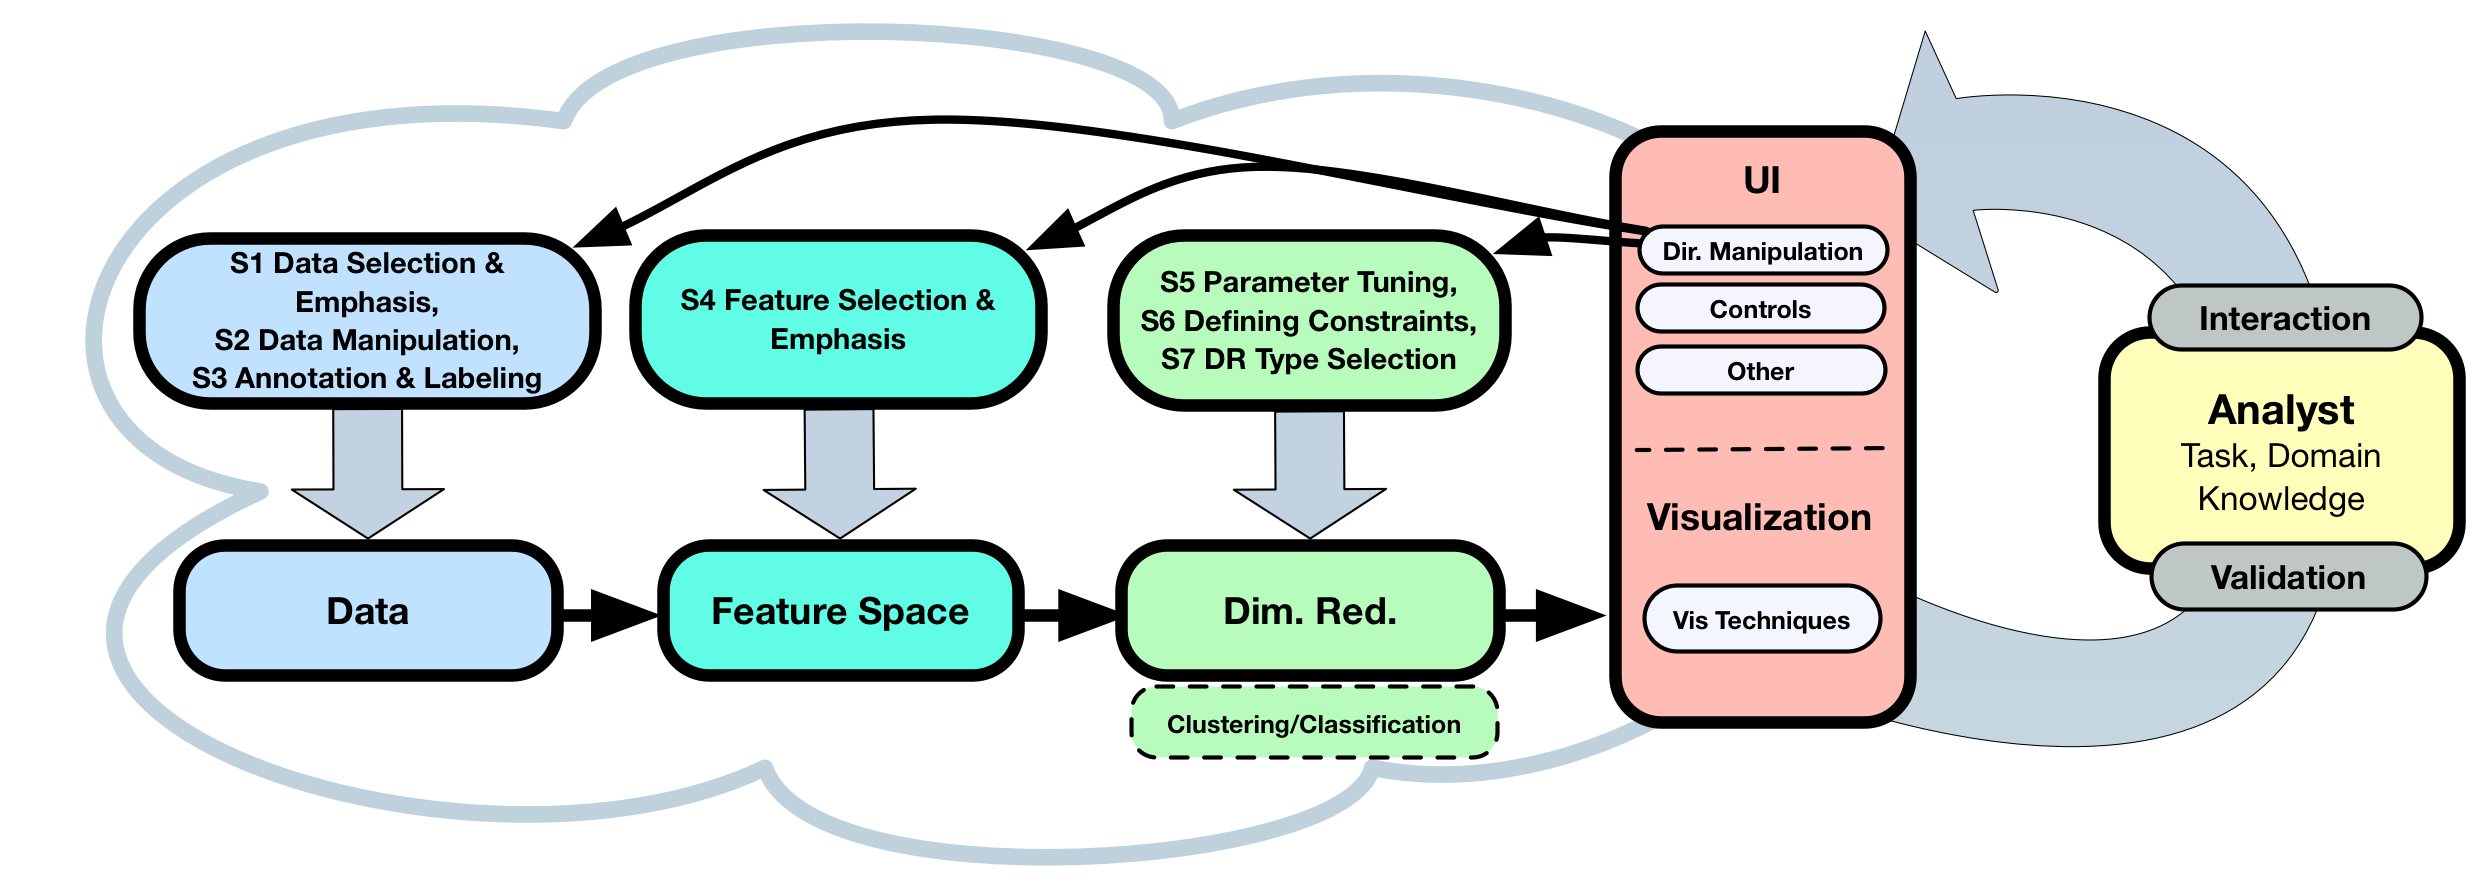
\includegraphics[width=0.9\linewidth]{Figures/dimred_framework.png}
    \caption{Human-in-the-loop process model proposed by \cite{Sacha2017-hf}. Included by permission.}
    \label{fig:sacha_fig}
\end{figure}

\citet{Venna2007-yj} discusses DR for ML and reviews many linear and non-linear projection methods. \citet{Vellido2012-nm} also discusses the importance of DR for making ML models interpretable. As one example, \citet{Chipman2005-om} applied this idea by constraining principle component analysis (PCA) in an attempt to make the resulting linear combinations of variables be more interpretable (more homogeneous, or more sparse).

At times a simple visualization is the most efficient way to communicate the results of decision making, planning. For example: \citet{Chadalavada2015-wx} enable a robot to project its path onto the ground so users can see.

\paragraph{Treatment of Uncertainty:}
In the previous section we have already visited the importance of an AIA being able to quantify its uncertainty. Visualization researchers are concerned with how to \emph{convey} that uncertainty to human users (and quantify uncertainty inherent in making visualizations). \cite{Sacha2016-tu} discuss how the propagation of uncertainty through visual analytics systems can affect the trust of human users (see also \cite{Correa2009-hi}).

One excellent example of this is the work by \citet{Wu2012-qi}, who create a tool to visualize the flow of uncertainty in the visualization process. In this way users can understand where uncertainty enters the visualization process.

\begin{figure}[htpb]
    \centering
    \includegraphics[width=0.6\linewidth]{example-image-golden}
    \caption{Example visualization of the flow of uncertainty in the creation of a visualization \cite{Wu2012-qi}. Included by permission.}
    \label{fig:hutchins_fig}
\end{figure}

The relationship between system uncertainty and the effects of uncertainty on the performance of the system can be very complex to understand. \citet{Hutchins2015-if} address this by using expert knowledge, and a `trust annunciator panel' (TAP) that has several `uncertainty level indicators' in order to display how uncertainties in sensors will effect the output quality, and the mission impact; and the same for the planning algorithm (see Figure~\ref{fig:hutchins_fig}).

\begin{figure}[htpb]
    \centering
    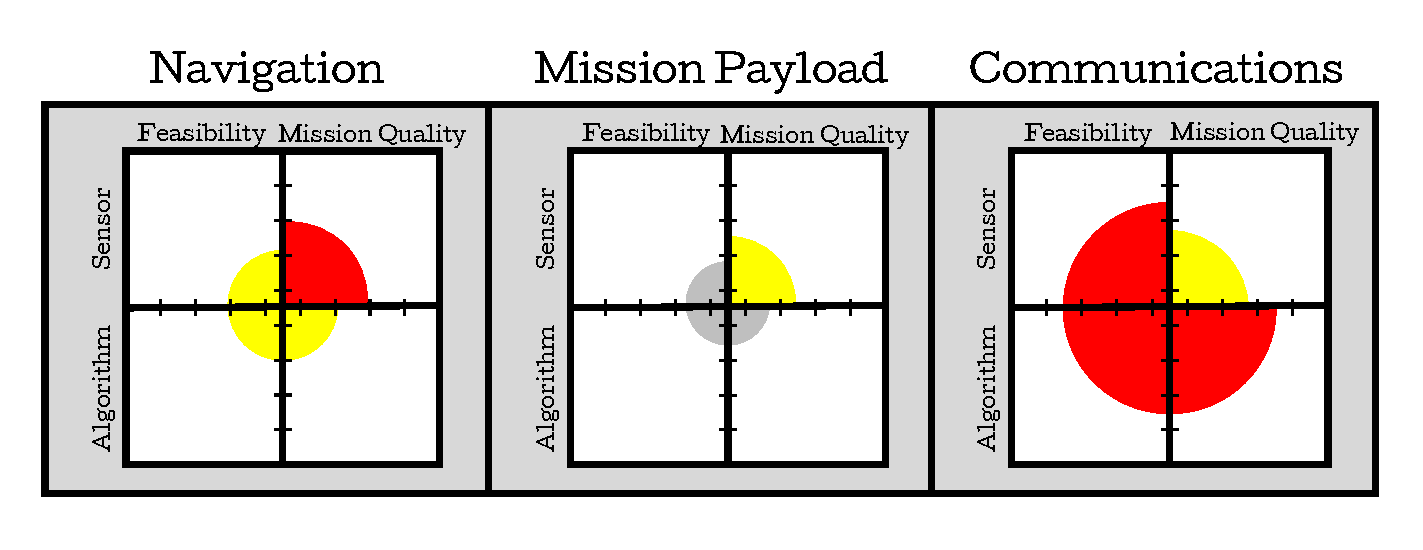
\includegraphics[width=0.9\linewidth]{Figures/Hutchins_fig.pdf}
    \caption{Proposed `trust annunciator panel' \cite{Hutchins2015-if}. Included by permission.}
    \label{fig:hutchins_fig}
\end{figure}

\subsubsection{Grounding Example:}
In the case of the `VIP Escort' problem (described in Section~\ref{sec:mot_example}), information visualization might be used as an assurance in the following way:

We make the following assumptions

\begin{itemize}
    \item The UGV has just begun an attempt to escape the road-network
    \item The user has access to an interface like that proposed in \cite{Hutchins2015-if}
\end{itemize}

During the attempt the user is able to see how the sensor uncertainty might possibly effect the outcome of the mission. In this case, the user is assured that the sensors will have little negative impact on the outcome of the mission given the current weather conditions.

\paragraph{\textbf{Discussion of Example:}} Here we see how a visualization is able to assist the user in correlating the effects between sensor uncertainty and mission outcome. This is not a simple relationship for operators (especially untrained) to learn on their own; even if they were able to learn the time required to do so can be very detrimental.
